\chapter{Introduction}
\label{cha:introduction}
This chapter provides the necessary background material and details the organization of my proposed work.

\section{Multi-modality}
\subsection{Modalities - Definition and Introduction}
\textit{Modality refers to the way something happens around us or is perceived by humans} \cite{Baltruaitis2017MultimodalML}. The world around us is composed of multiple sensory modalities, as listed below, with enabled capabilities:
\begin{itemize}
    \item \textbf{Visual:} Watching objects and events in the current visual scene
    \item \textbf{Language:} Verbal interactions with other humans 
    \item \textbf{Audio:} Speaking and hearing environmental sounds 
    \item \textbf{Touch:} Feeling texture of objects 
    \item \textbf{Smell:} Distinguishing between pleasant and unpleasant odors.
\end{itemize}
For humans, the information from multiple sensory sources is processed by distinct regions of the brain for different perceptual tasks \cite{Alain2001WhatA,BornkesselSchlesewsky2015NeurobiologicalRO,Wallace2002HistochemicalIO}. While the visual input processing is handled by the occipital lobe in the brain, the auditory and language inputs are processed by specific regions of the temporal lobe. The sub-division of the human neural processing system into regions that can process a wide variety of modalities indicates the heterogeneity among different sources along with underlying commonalities, as shown in Fig \ref{}.

\begin{figure}
    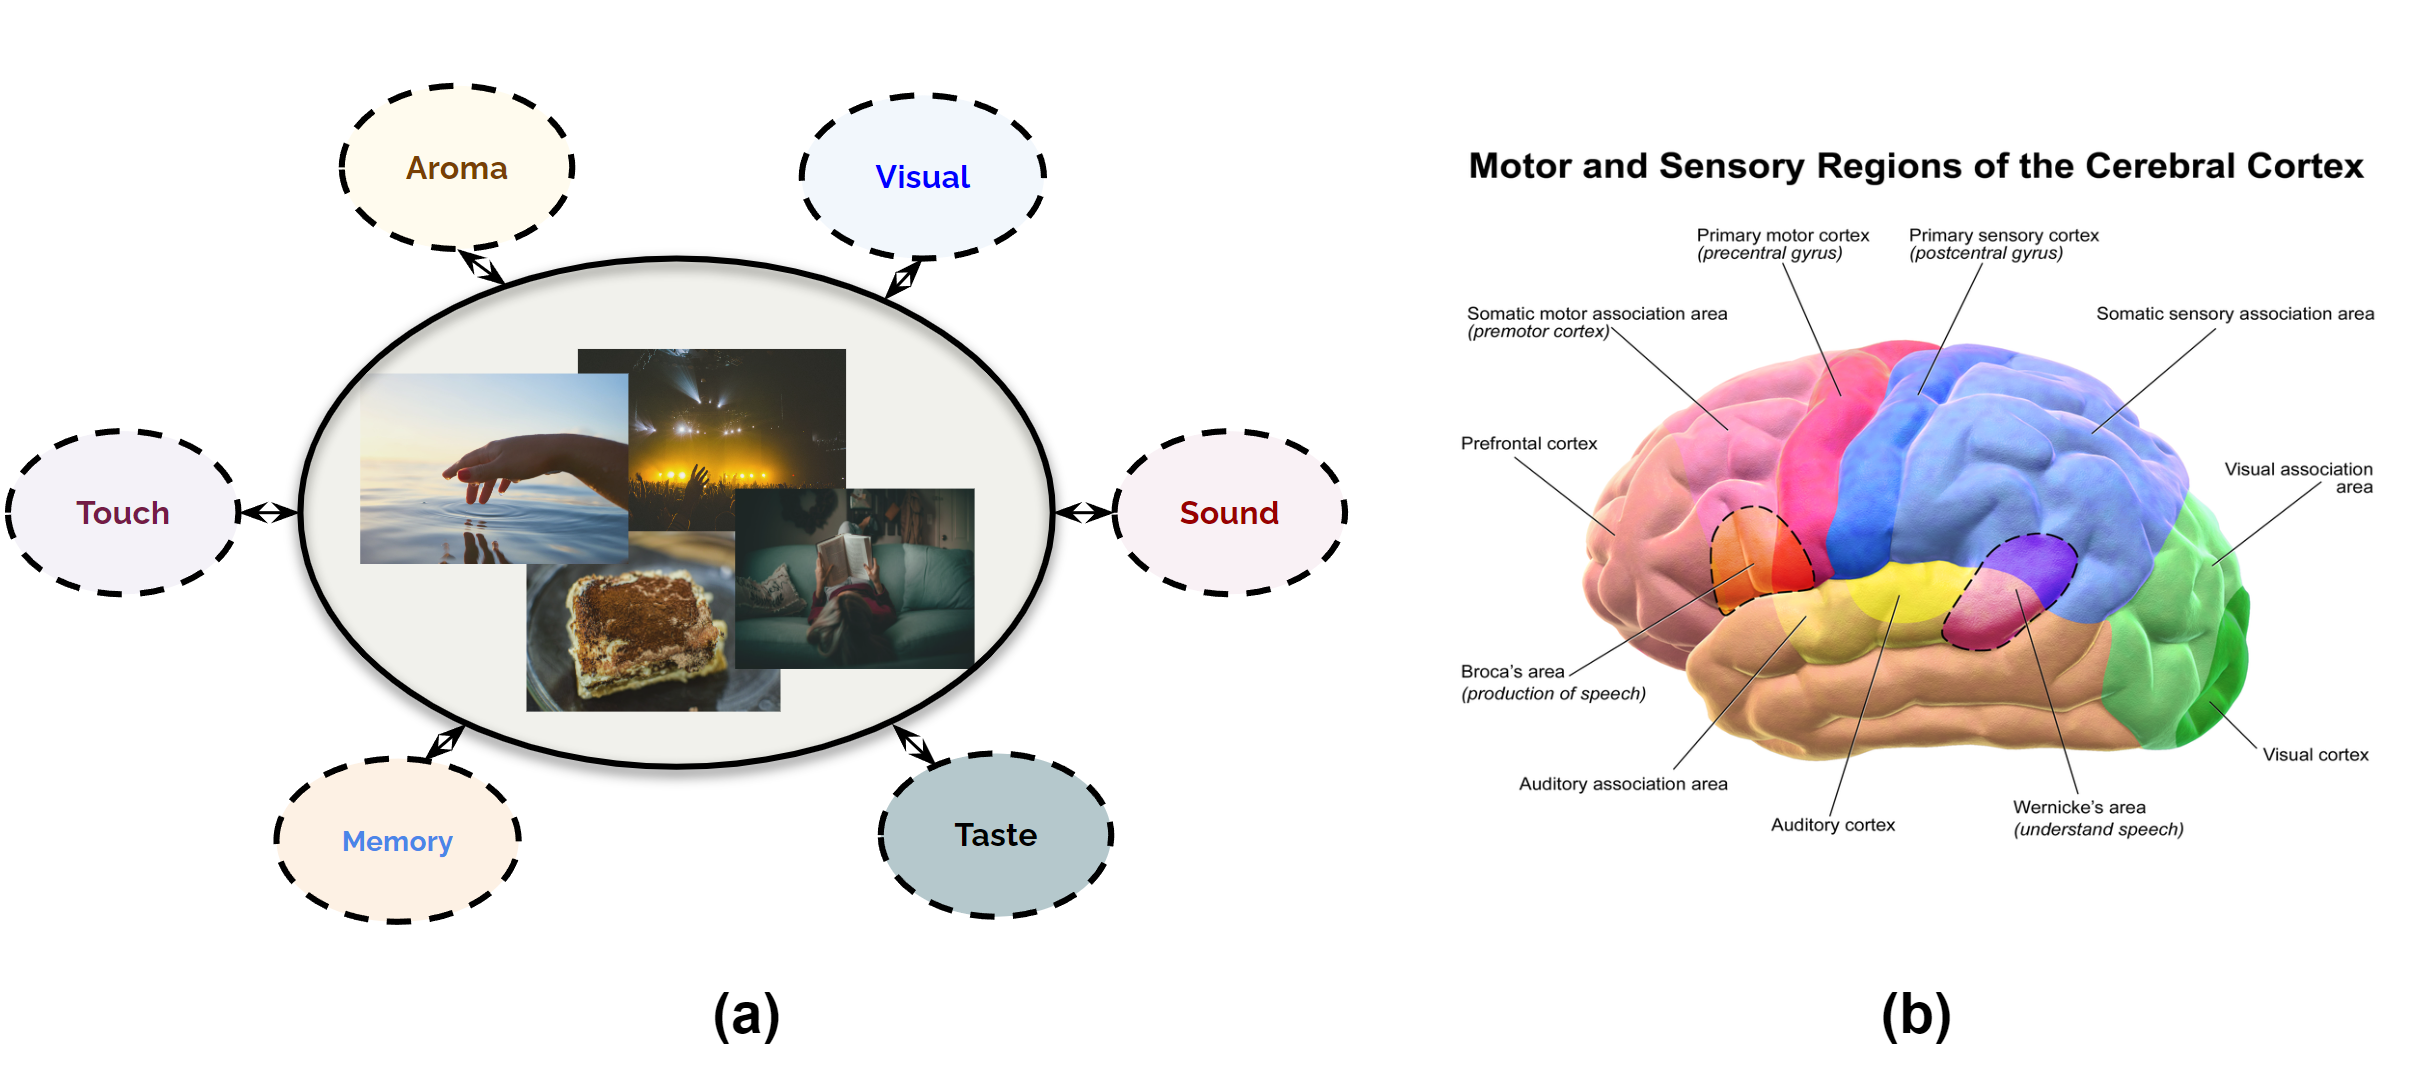
\includegraphics[width=\textwidth]{figures/cererbral_cortex_multiple_modalities.png}
    \caption{ (a)  Sensory modalities associated with real-world human perception  (b)  Specialized regions in brain where sensory information comes together and processed by different cortices}
\end{figure}

In artificial intelligence, a given task is considered multi-modal if multiple sensory modalities are needed to solve the same. The goal of artificial intelligence is to develop autonomous agents that can learn from diverse input modalities to solve complex reasoning tasks. As mentioned by Liang et al. \cite{Liang2022FoundationsAR}, the key properties associated with learning from multimodal data are listed as follows:
\begin{itemize}
    \item \textbf{Heterogeneity:} Heterogeneous nature of different modalities due to diversity in qualities, structures, and representations
    \item \textbf{Connectedness:} Shared/common information between different modalities due to inter-related nature.
    \item \textbf{Interaction:} Existence of optimal interactions/fusions between different modalities, suitable for particular task.
\end{itemize}
Based on the above properties associated with multiple modalities, the major challenges in multimodal learning \cite{Liang2022FoundationsAR} can be summarized below:

\begin{itemize}
    \item \textbf{Representation:} Learning representations through fusion mechanisms that capture the heterogeneity of the modalities along with the shared information. For example, language is considered symbolic due to its word-based composition, whereas audio and visual modalities are represented through signals.
    \item \textbf{Alignment:} Identifying relationships between (sub) elements of different modalities. This requires similarity computation between different modalities along with the handling of long-term dependencies.
    \item \textbf{Reasoning:} Combining knowledge from multiple sources (including external, i.e. knowledge graphs) in a multi-step inference process by exploiting the task structure.
    \item \textbf{Generation:} Translating between different modalities and summarization of multimodal data by preserving the salient content.
    \item \textbf{Transference:} Transferring cross-modal knowledge from secondary modalities to the primary modality in the presence of noise or limited data.
\end{itemize}

% In this work, we deal with the alignment, reasoning, and transference challenges associated with multi-modal learning.
    
\subsection{Rise of multi-modal content}

With the rapid rise in heterogeneous internet networks across the globe, vast amounts of web-based content have been generated at different scales, variety, and velocity \cite{Gao2020ASO}. Web-based sources convey information to the viewers through a combination of multiple modalities. For example, an online news article about a major sports event contains text descriptions with accompanying images. Further, the movies or TV shows hosted through online streaming platforms portray narratives through the combination of video and audio signals (music, speech, ambient sounds). 
The demand for media content, especially movies, TV shows, and advertisements, is expected to rise over the next three years, with the projected market value to reach 2.9 trillion US dollars, as shown in Fig \ref{media industry demand}.
\begin{figure}[h!]
    \centering 
     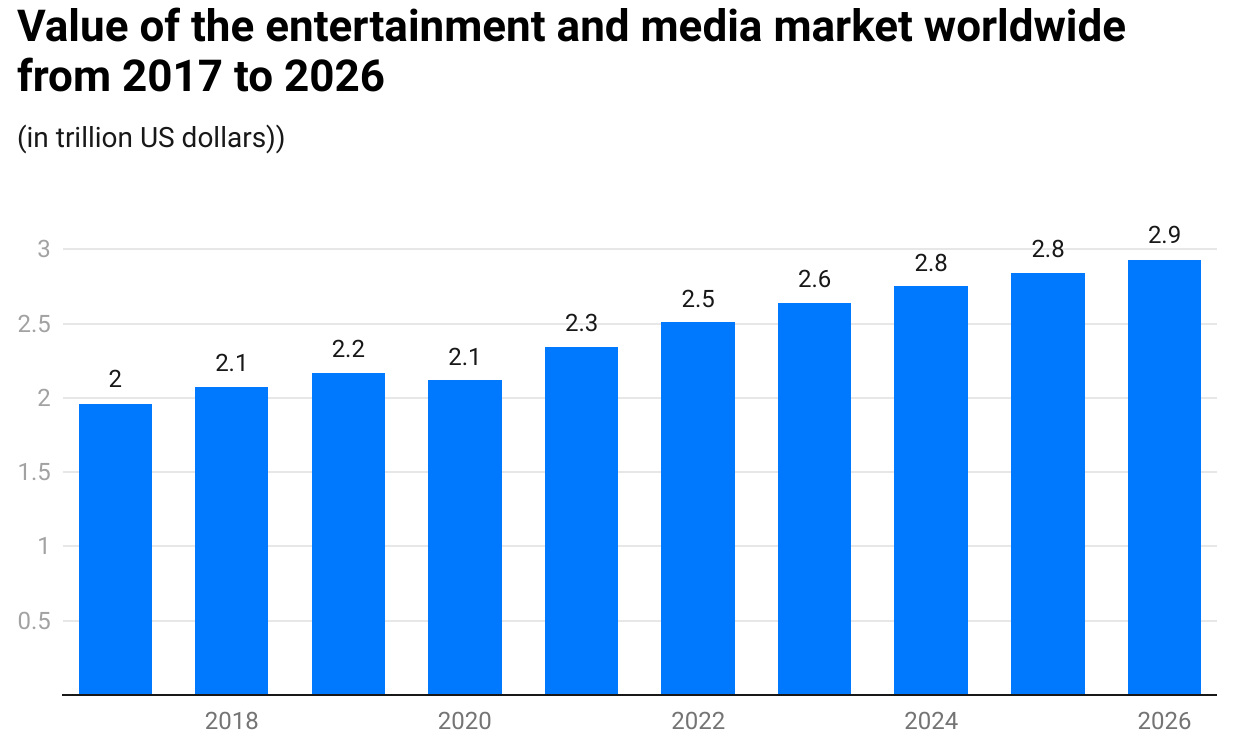
\includegraphics[width=0.6\linewidth]{figures/media_industry_demand.png}
     \caption[Media value]{Expected value of entertainment market industry from 2017 to 2026 \footnotemark} 
     \label{media industry demand}
\end{figure}
\footnotetext{\url{https://www.enterpriseappstoday.com/stats/media-and-entertainment-industry-statistics.html}}
The growing demand for multi-modal media content has led to various descriptive tasks such as captioning \cite{Abdar2023ARO}, video summarization \cite{Apostolidis2021VideoSU}, and question-answering \cite{defaria2023visual}, aimed at enhancing user experience. In the following sections we will introduce the concept of context and how multiple modalities provide contextual information.

\section{What is context ?}
In computer vision, context \cite{contextvision} refers to any relevant information encompassing the attributes of the object and event considered, along with other entities (objects and events) in the given scene, both visual and non-visual. Contextual information enables a wide variety of tasks, including object recognition, human affect perception, and salient event detection in videos, by providing additional cues needed for accurate inference. For example, the visual scene in a given image provides the necessary contextual information to detect commonly co-occurring objects along with any atypical placements. In terms of object placements, utensils are more likely to be found in the kitchen as compared to bedrooms or stadiums. An example of context providing the required information to improve object recognition under challenging conditions (poor lighting, image blurring, ) is shown in Fig \ref{object recognition}. The blurred object (marked by a red circle), when viewed in isolation, is not recognizable. However, when the object is placed in the context of the entire visual scene i.e. office, we can see that it is likely to be a keyboard.
\begin{figure}
    \centering 
     
\includegraphics[width=0.6\linewidth]{figures/blurred_object.png}
     \caption{ \textbf{LEFT:} A blurred object (marked in red circle), when viewed in isolation, is not recognizable. \textbf{RIGHT:} Contextual information in the form of the visual scene helps in recognition. Image source: \cite{Marques2010ContextMI}}
     \label{object recognition}
\end{figure}

The broad organization of different context sources, along with associated levels is shown in Fig \ref{Context_type}.
\begin{figure}[t]
  \centering
  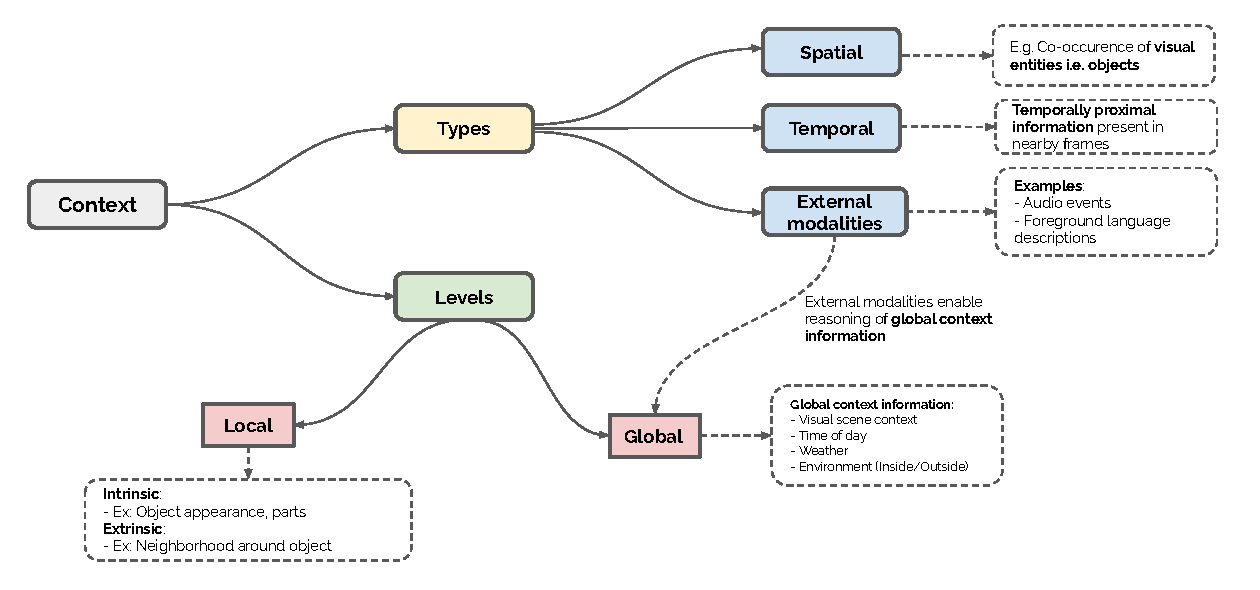
\includegraphics[width=\linewidth]{figures/Context_type.pdf}
  \caption{Variations in types and levels of context. Outline of context levels and types inspired from Fig 5 in \cite{contextvision}.}
  \label{Context_type}
\end{figure}
Context can be broadly divided into three types as follows:

\subsection{Spatial context}
Spatial context refers can be defined as the \textit{possibility of finding objects located at certain positions in the scene w.r.t other proximal objects}. For example, a ship can be found floating at sea rather than on a highway.
Spatial context can be further subdivided into the following major classes:
\begin{itemize}
    \item  \textbf{Spatial co-occurrence}: Spatial co-occurrence can be leveraged through co-occurrences of object labels in the same visual scene. Rabinovich et.al \cite{Rabinovich2007ObjectsIC} utilized co-occurrence statistics between labels in a CRF-based framework to refine object detections in a given visual scene. Further, Wang et al. \cite{Wang2007ShapeAA} expanded the idea of co-occurrence by providing a probability distribution of labels over different regions based on a given pixel location. Yang et.al \cite{Faceness-Net} explored fine-grained relative spatial information between facial parts i.e., placement of nose, mouth for face detection. 
    \item  \textbf{Direction and toplogical relations}: 2-D spatial relations between entities can be described through direction and topological-based relations \cite{Marques2010ContextMI}. Directional relations deal with the proximity of one object with other objects in terms of other entities based on relative terms like \textit{"near"}, \textit{"above"}, \textit{"below"}. Whereas topological relations are concerned with the neighborhood of the objects in terms of overlap/containment with distinct regions i.e. exterior, boundary and interior.
    \item  \textbf{Semantic driven spatial context}: Semantic context restricts the space of possible spatial contextual relations in a given scene to a set of valid ones. The usage of semantic context between proximal objects enables correction of mislabeling in images \cite{Rabinovich2007ObjectsIC}, and accurate discovery of all possible valid relations between objects through scene graphs \cite{Chang2021ACS}. An example of a scene graph with entities and semantic relations obtained after message-passing operations \cite{Xu2017SceneGG} is shown in Fig \ref{scenegraph}.
    \begin{figure}[h!]
    \centering
        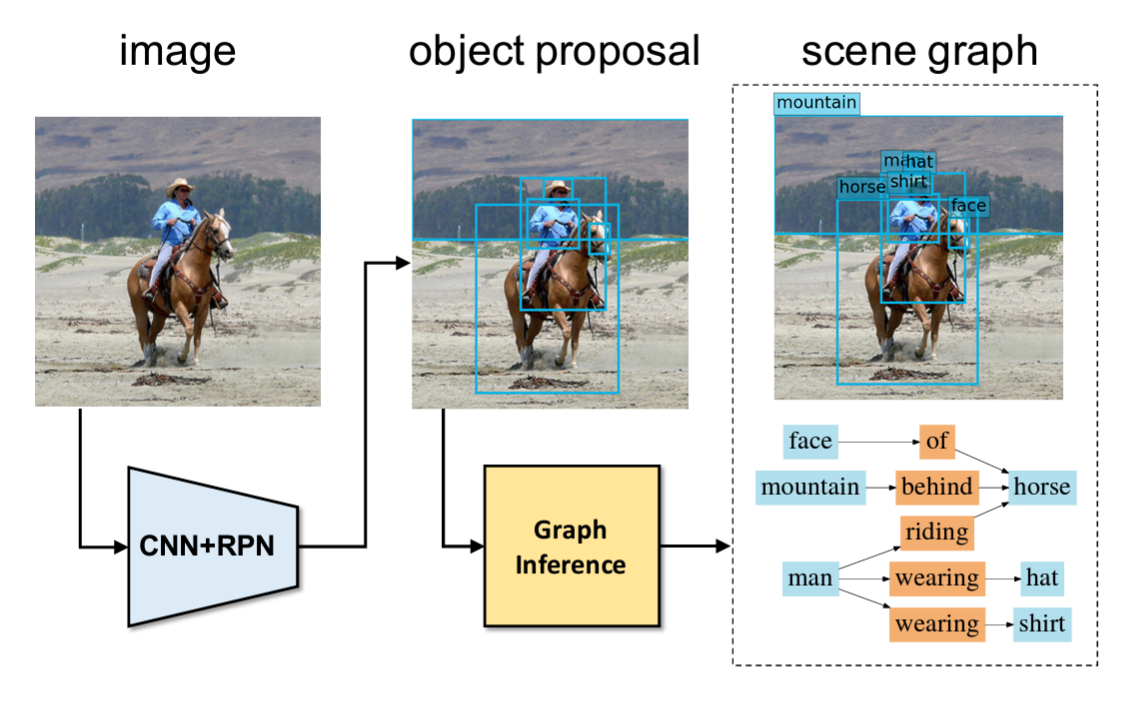
\includegraphics[width=0.5\linewidth]{figures/Scene_graph_outline.png}
        \caption{Sample scene graph obtained after iterative message passing (graph interface) over the region proposals (objects) }
        \label{scenegraph}
    \end{figure}
\end{itemize}

\subsection{Temporal context}
Temporal context refers to the \textit{information present in dynamic content, i.e. nearby or distant frames in videos}. The major subdivisions of temporal context are listed as follows:
\begin{itemize}
\item \textbf{Short-term temporal context:} Short-term temporal context relies on information present in nearby frames, which can be a short temporal window centered on the current frame or previous frame. The temporal context within a short window, (usually a few seconds) enables general video understanding tasks, including action recognition \cite{Carreira2017QuoVA}, pedestrian tracking \cite{Yan2019LearningCG}, human-object interaction \cite{Ji2021DetectingHR}. 
\item \textbf{Long-term temporal context:} Instead of limiting to nearby frames, long-term temporal context deals with temporal scale spanning from hours to months/years. General media-focused tasks based on movies \cite{Wu2021TowardsLV,Soldan2021MADAS} rely on long-form narratives (usually minutes to hours) for understanding character interactions, event dynamics, and broad semantics, including genre, etc. For tasks like species monitoring, temporal information over extended periods of time (months or years) is required for accurate identification \cite{Beery2019ContextRL}. 
\end{itemize}
In spite of clear divisions between short-term and long-term temporal contexts based on the duration of information, certain narrative-driven videos in media, i.e., advertisements, contain: 
\begin{itemize}
\item Rapid changes in short-term contextual information based on shots. 
\item Long-term contextual association between the shots based on an integrated narrative.
\end{itemize}
\subsection{External modalities}
Apart from visual-only information, modalities such as audio, language, and prior weather information also provide relevant contextual information for various reasoning tasks. For example, in the case of audio-visual tasks, the audio associated with an entity, i.e., dog barking, can help us estimate the proximity of the sound source and localize it in the given video \cite{Tian2018AudioVisualEL}. Further usage of audio modality as an additional contextual source for visual tasks has been explored in floorplan design \cite{purushwalkam2020audio} and audio-visual navigation for virtual agents \cite{chen2020soundspaces}. For various vision-language tasks like temporal grounding, natural language queries can be used as contextual inputs to isolate regions of interest in unconstrained videos \cite{Zhang2022TemporalSG}. Besides language and audio, additional contextual information available through thermal sensors \cite{Seymour2017AutomatedDA} is used to augment the visually captured data for improving wildlife detection in remote areas. In case of affect understanding problems, multi-turn dialogues (\textbf{language modality}) provide the necessary context information (i.e. topics and flow of information) along with facial expressions for emotion tracking of the speakers \cite{Zhao2022M3EDMM}.

\subsection{Local context}
Local context refers to the \textit{contextual information associated with objects itself (\textbf{intrinsic}) and surrounding local regions (\textbf{extrinsic}) such as color, shape, contrast, aspect ratio} \cite{contextvision}. Local context is closely related to spatial information in terms of the immediate neighborhood of the objects in the scene. Effective utilization of local context enables the detection of small objects in complex scenes with multiple entities. External modalities often provide local context for multi-modal reasoning, i.e., the conversation history (\textbf{language}) enables the autonomous agent associated with visual dialog \cite{Das2016VisualD} to provide the correct in-context answer.

\subsection{Global context}

Global context utilizes \textit{the overall configuration of the scene as a source of contextual information \cite{contextvision}}. The primary sources of global context information are as follows:
\textbf{(A) Visual scene:} The visual scene where the objects are present, i.e. living room, kitchen, train station etc. \\
\textbf{(B) Time of day:} The timing shown in the given image/video i.e. day, night, evening, or morning. \\
\textbf{ (C) Weather:} The ambient weather conditions associated with the given scene, i.e. sunny etc. \\
\textbf{ (D) Environment:} The environment associated with the given scene i.e., inside or outside.
\par 
Visual scene, along with the associated environment provides the prior context for finding certain objects. For example, there is a greater likelihood of finding utensils in the kitchen (\textbf{indoor visual scene}) as compared to train station (\textbf{outdoor visual scene}). Global context information (in the form of visual scenes) also influences the relative placement of different objects, like the proximity of a keyboard to the monitor in an office setup. Further, the accurate identification of different objects as part of the local contextual information in a given image/video can also help 
in recognizing the given visual scene \cite{Torralba2003ContextualPF} and its attributes (i.e., indoor/outdoor, time of day, etc.). For example, the presence of a microwave oven and dishwasher indicates that the visual scene is likely a kitchen. The global context information can also help in identifying atypical scenarios \cite{Choi2012ContextMA} involving objects i.e., a car located in the sky or a plane running on a highway, as shown in Fig \ref{outcontext}. 

\begin{figure}[h!]
    \centering
        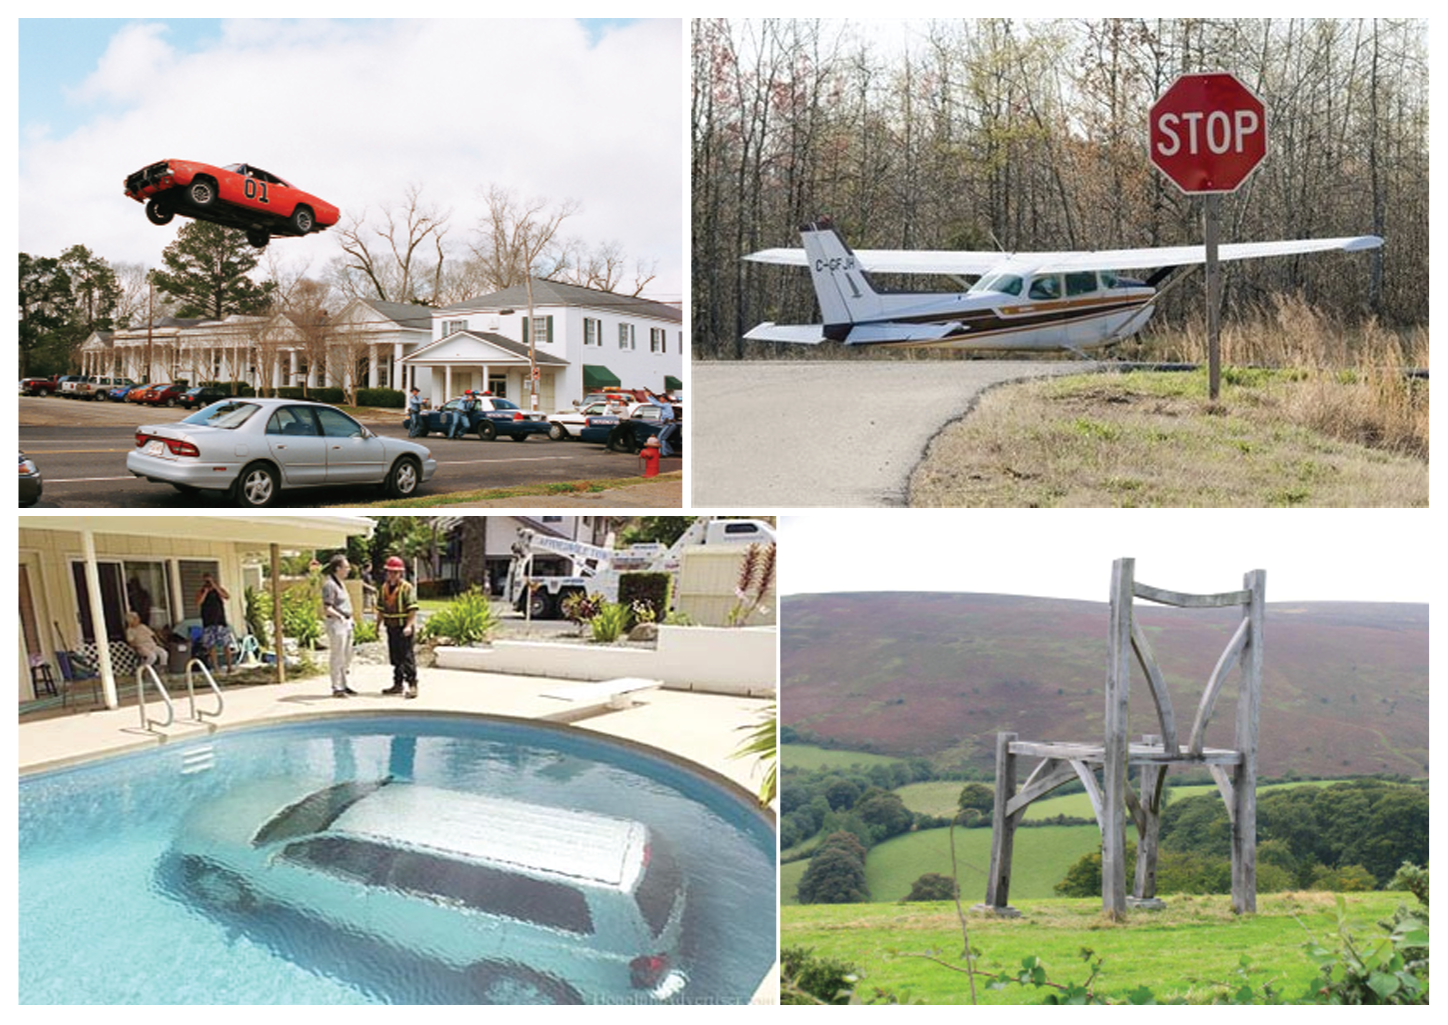
\includegraphics[width=0.5\linewidth]{figures/out_of_context_image.png}
        \caption{Sample images from \cite{Choi2012ContextMA} showing atypical scenarios involving violations of support, position, probability, size }
        \label{outcontext}
\end{figure}
    
\section{Context-driven multi-modal understanding}

\begin{figure}[h!]
    \centering
        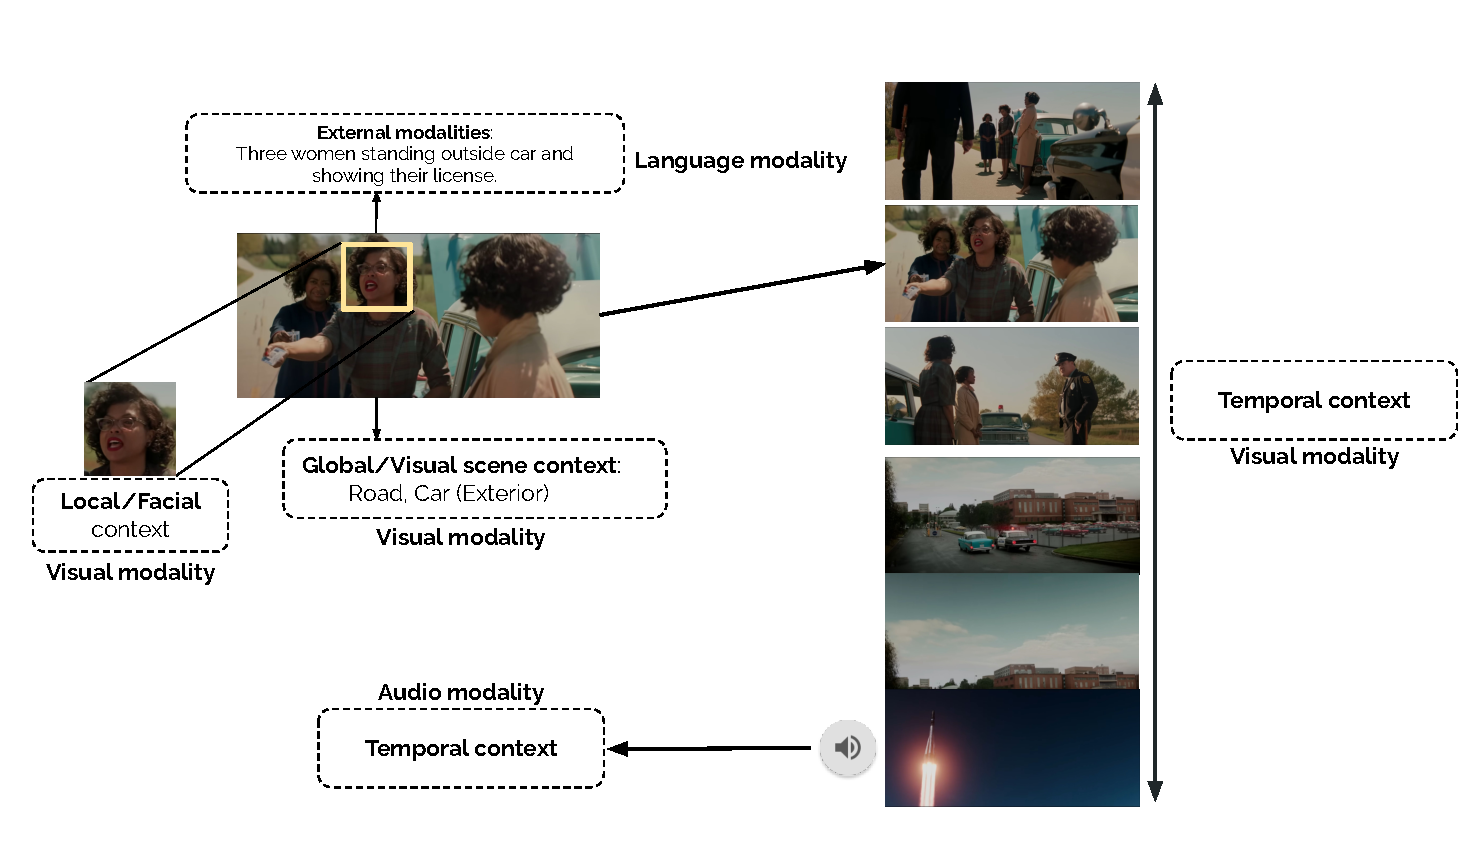
\includegraphics[width=0.9\linewidth]{figures/context_diagram.pdf}
        \caption{Outline diagram showing the presence of various contexts and associated modalities in a sample movie clip.} 
        \label{contextmultimodal}
\end{figure}


Multi-modal tasks require the processing of diverse contextual information followed by fusion for both macro and instance-level content understanding. In the case of multi-modal content, the contextual information is usually obtained through multiple input modalities. In \textbf{Fig \ref{contextmultimodal} (a)} \footnote{Hidden Figures (2016): https://www.youtube.com/watch?v=W1VZ1-ZdQ7k\&ab\_channel=20thCenturyStudios}, we can see that the face crop of the person captures the \textbf{local/facial} context in the frame of interest. The \textbf{global} context is captured by visual scene i.e., \textbf{road, car (exterior)}. External modalities in the form of natural language descriptions, i.e., \textit{Three women standing outside the car and showing their license} provide information about the interactions happening in the foreground. Further, this frame is a part of a longer narrative, as shown in the sequence of frames. The frame sequence captures both short-term and long-term \textbf{temporal context}, where short-term context centers around local activities, including interactions between the woman and the policeman, followed by long-term temporal context involving multiple transitions within the narrative. By taking long-term temporal context into account, it can be seen that the clip ends with a spacecraft launch. Further, the sound event associated with spacecraft launch captures additional short-term temporal context.


\section{Multimodal content understanding - scale}

This work considers multimodal content understanding at two distinct scales: \textbf{instance-level} and \textbf{macro-level}. 

\subsection{Macro-level content understanding}
Macro level provides an expanded view by referring to the broad thematic elements associated with multimodal content like \textit{broad theme/topic}, \textit{underlying genre}, \textit{sentiment}, etc. As seen in Fig \ref{macro_scale_understanding} (a), the broad theme/topic, i.e., \textbf{Performing arts}, provides the macro-level view of the video. Further in Fig  \ref{macro_scale_understanding} (b), the genre, i.e., \textbf{animation}, \textbf{action}, \textbf{adventure} gives a high-level insight into the movie snippet. In our work, we consider macro-level understanding along the lines of genre for movie trailers and broad thematic elements for advertisement videos. 
\begin{figure}
 \centering
    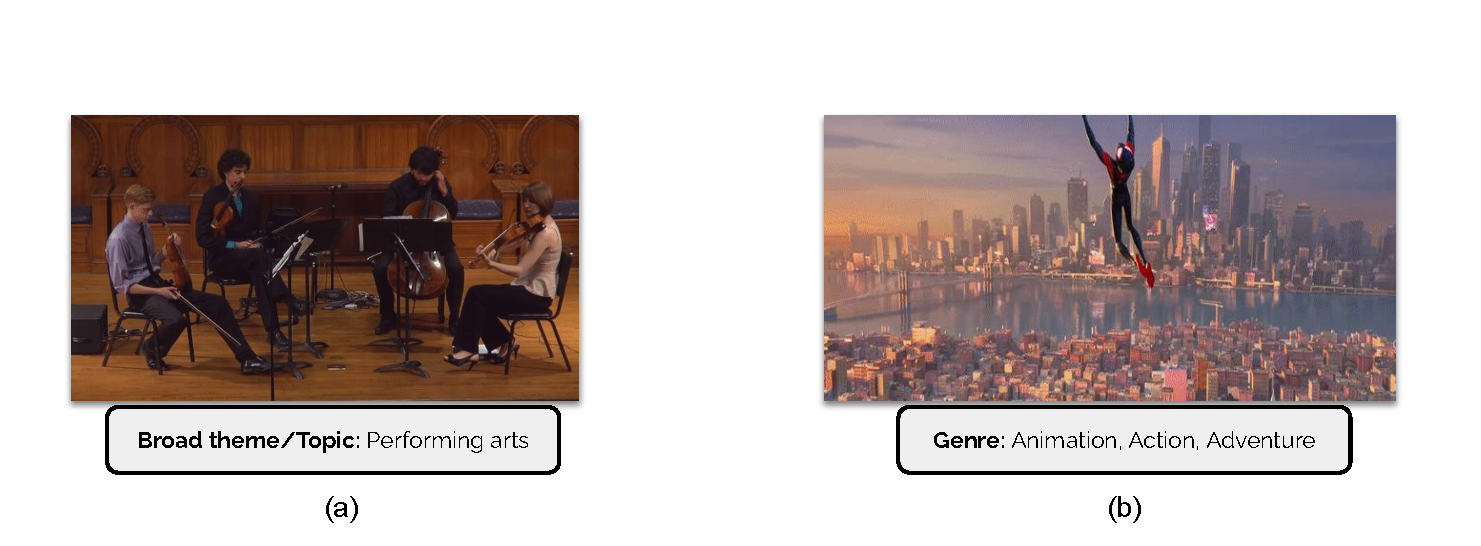
\includegraphics[width=\textwidth]{figures/macro_scale_understanding.pdf}
    \caption{Macro-level understanding examples (a) \textbf{Broad theme/topic:} Performing arts (b) \textbf{Genre:} Animation/action/adventure}
    \label{macro_scale_understanding}
\end{figure}

\subsection{Instance-level content understanding}

Instance level refers to content understanding at the scale of individual entities like objects and persons w.r.t. different attributes like \textbf{appearance}, \textbf{perceived emotional state}, \textbf{gender}, \textbf{age}, \textbf{skintone} and \textbf{occupation}. For example, in Fig \ref{instance_scale_understanding} (a) and (b), the instance-level view refers to the person with the green bounding box and the associated attributes of perceived age, gender, and affective state. In our work, we look at instance-level content understanding in terms of estimating the affective state of the person.

\begin{figure}
 \centering
    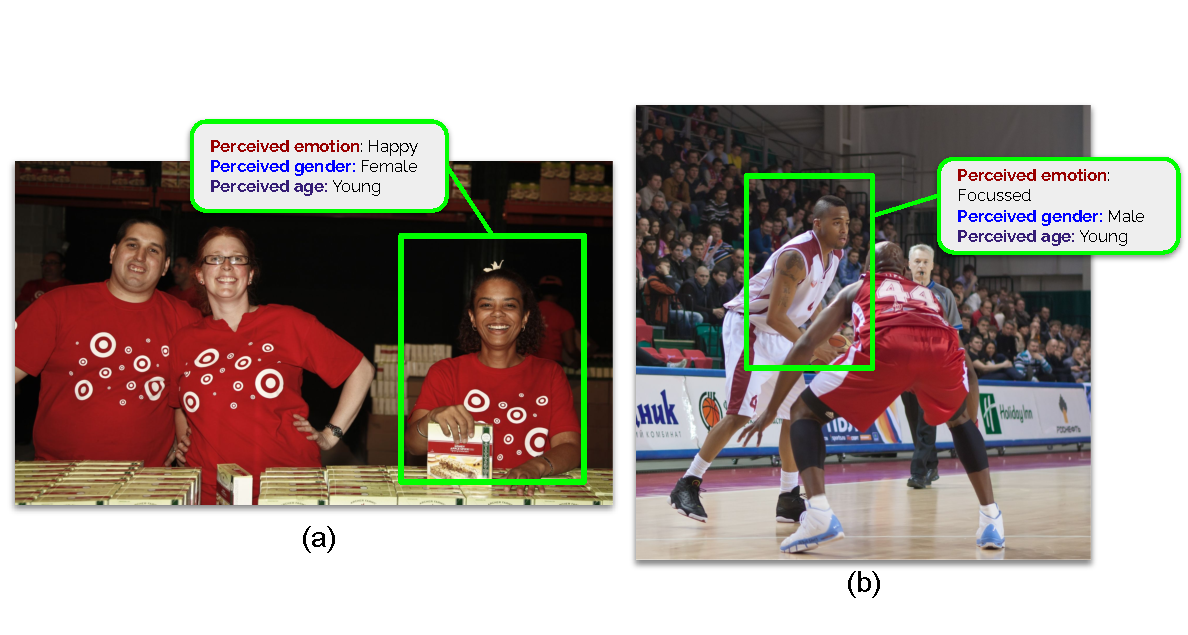
\includegraphics[width=\textwidth]{figures/instance_level_scale_understanding.pdf}
    \caption{Instance-level understanding examples}
    \label{instance_scale_understanding}
\end{figure}


\section{Organization of proposal}

\begin{figure}[h!]
    \centering
        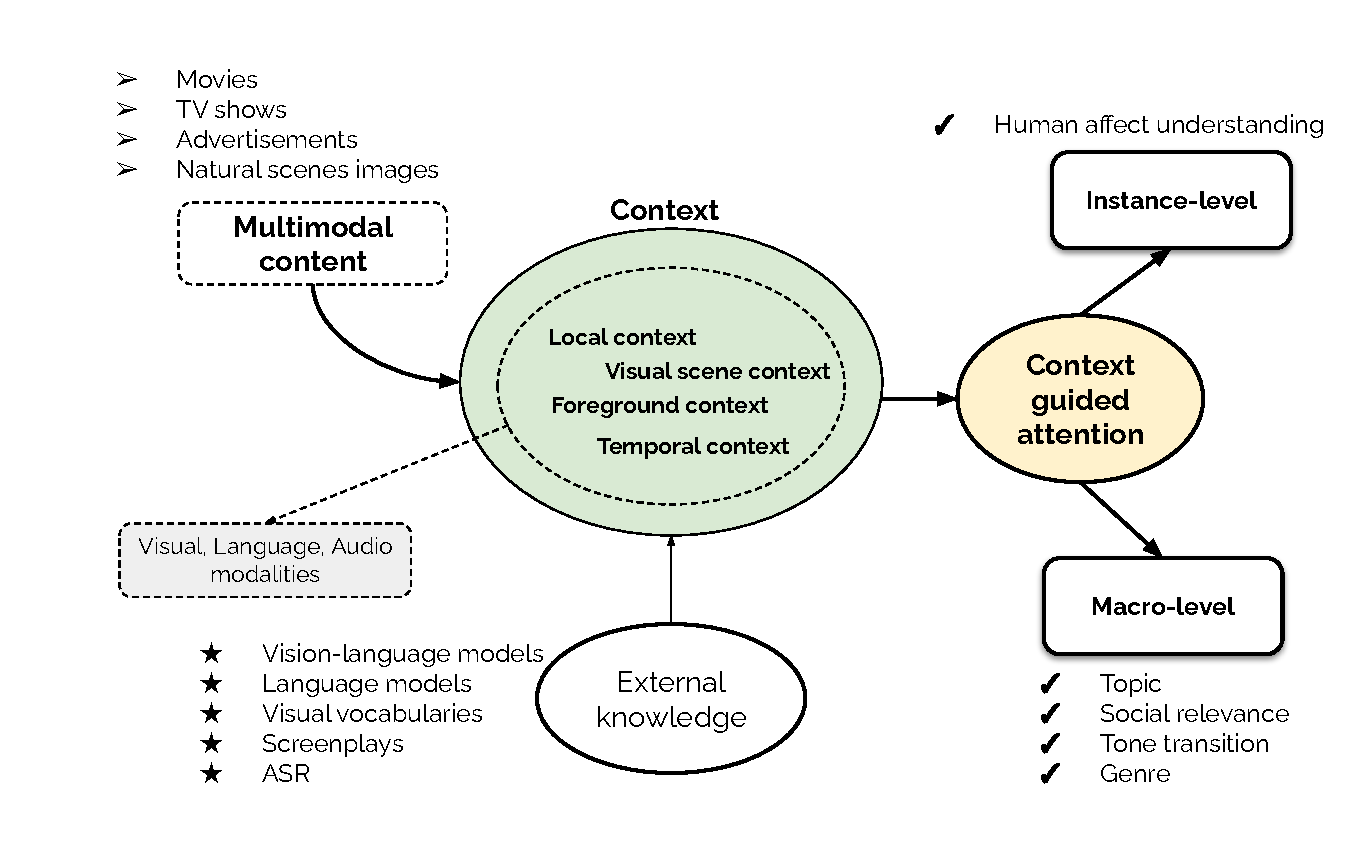
\includegraphics[width=\textwidth]{figures/Overview_diagram.pdf}
        \caption{Organization of the thesis proposal with different components}
        \label{proposalorganization}
\end{figure}

In this section, we provide the basic outline of the thesis proposal. The proposed thesis statement is given as follows:

\begin{tcolorbox}[width=\textwidth]
Context-guided attention improves multi-modal content understanding at diverse scales.
\end{tcolorbox}


We develop contextual approaches for improved multimodal content understanding at different scales: \textbf{instance-level} and \textbf{macro-level}.  In terms of input sources, we consider multi-modal media content, including \textbf{movies}, \textbf{TV shows}, \textbf{advertisements}, and \textbf{natural scene images}. Looking at the multimodal content from both instance and macro-level viewpoints provides a holistic understanding of given inputs. In terms of the distinction between context and modalities, we use modalities available in input sources to extract diverse forms of contextual information. Further, dissimilar modalities can provide similar types of contextual information. For example, both visual and audio modalities provide the necessary temporal context for various content-understanding tasks. An outline of the proposal is shown in Fig \ref{proposalorganization}, showing the relationships between input multimodal content and content understanding at different scales. \textbf{[External knowledge]}.For processing the contextual information, we propose context-guided attention mechanisms \textbf{[ADD HERE]}



We consider multi-modal media content, including \textbf{movies}, \textbf{TV shows}, \textbf{advertisements}, and \textbf{in-the-wild} videos as the primary input sources for exploration. Since multi-modal media content is curated with the aim of portraying human-centered narratives \cite{CMI}, our focus is to obtain both \textbf{instance-level} and \textbf{macro-level} insights by combining multiple contextual signals in a multi-modal learning framework. As shown in Fig \ref{proposalorganization}, the contextual information is obtained through input multiple modalities as follows:

\begin{itemize}
    \item  \textbf{Visual modality:} Captures \textbf{\textit{spatial/temporal context}} through visual semantic units i.e., objects, and persons captured over images and videos.
    \item  \textbf{Language modality:} Captures \textbf{\textit{spatial context (semantic)}} through foreground based natural language descriptions of images.
    \item  \textbf{Audio modality:} Captures \textbf{\textit{temporal context}} through audio events, background music and speech.

\end{itemize}
Apart from the input modalities, we also consider external pretrained knowledge from multimodal models (obtained through web-scale data) as expert inputs.
We combine the above-mentioned inputs in a content understanding framework in the following sequence of chapters:

\begin{enumerate}
    \item \textbf{Chapter 2}: We explore the problem of global context reasoning in the form of visual scene context from multi-modal data esp. movies, by leveraging external knowledge from pretrained multimodal model i.e., CLIP \cite{Radford2021LearningTV}.
    \item \textbf{Chapter 3}: We utilize our insights from Chapter 1 to propose a multimodal context fusion approach for contextual human affect (\textbf{instance-level}) understanding in natural scenes and TV shows.
    \item \textbf{Chapter 4}: We explore the fusion of spatial and temporal context through multiple input modalities for macro-level understanding in advertisement videos having dynamic contextual changes. 
    \item \textbf{Chapter 4}: We propose an efficient information-theoretic framework to fuse contextual information in multimodal pretrained transformers for multi-scale content understanding tasks.
\end{enumerate}

\textbf{Chapter 5} is an ongoing work and will be extended into post-proposal for integration into final thesis dissertation.
